\documentclass{article}

\usepackage[a3paper]{geometry}
\usepackage{tikz}
\usepackage{lscape}
\usetikzlibrary{automata, positioning}
\begin{document}
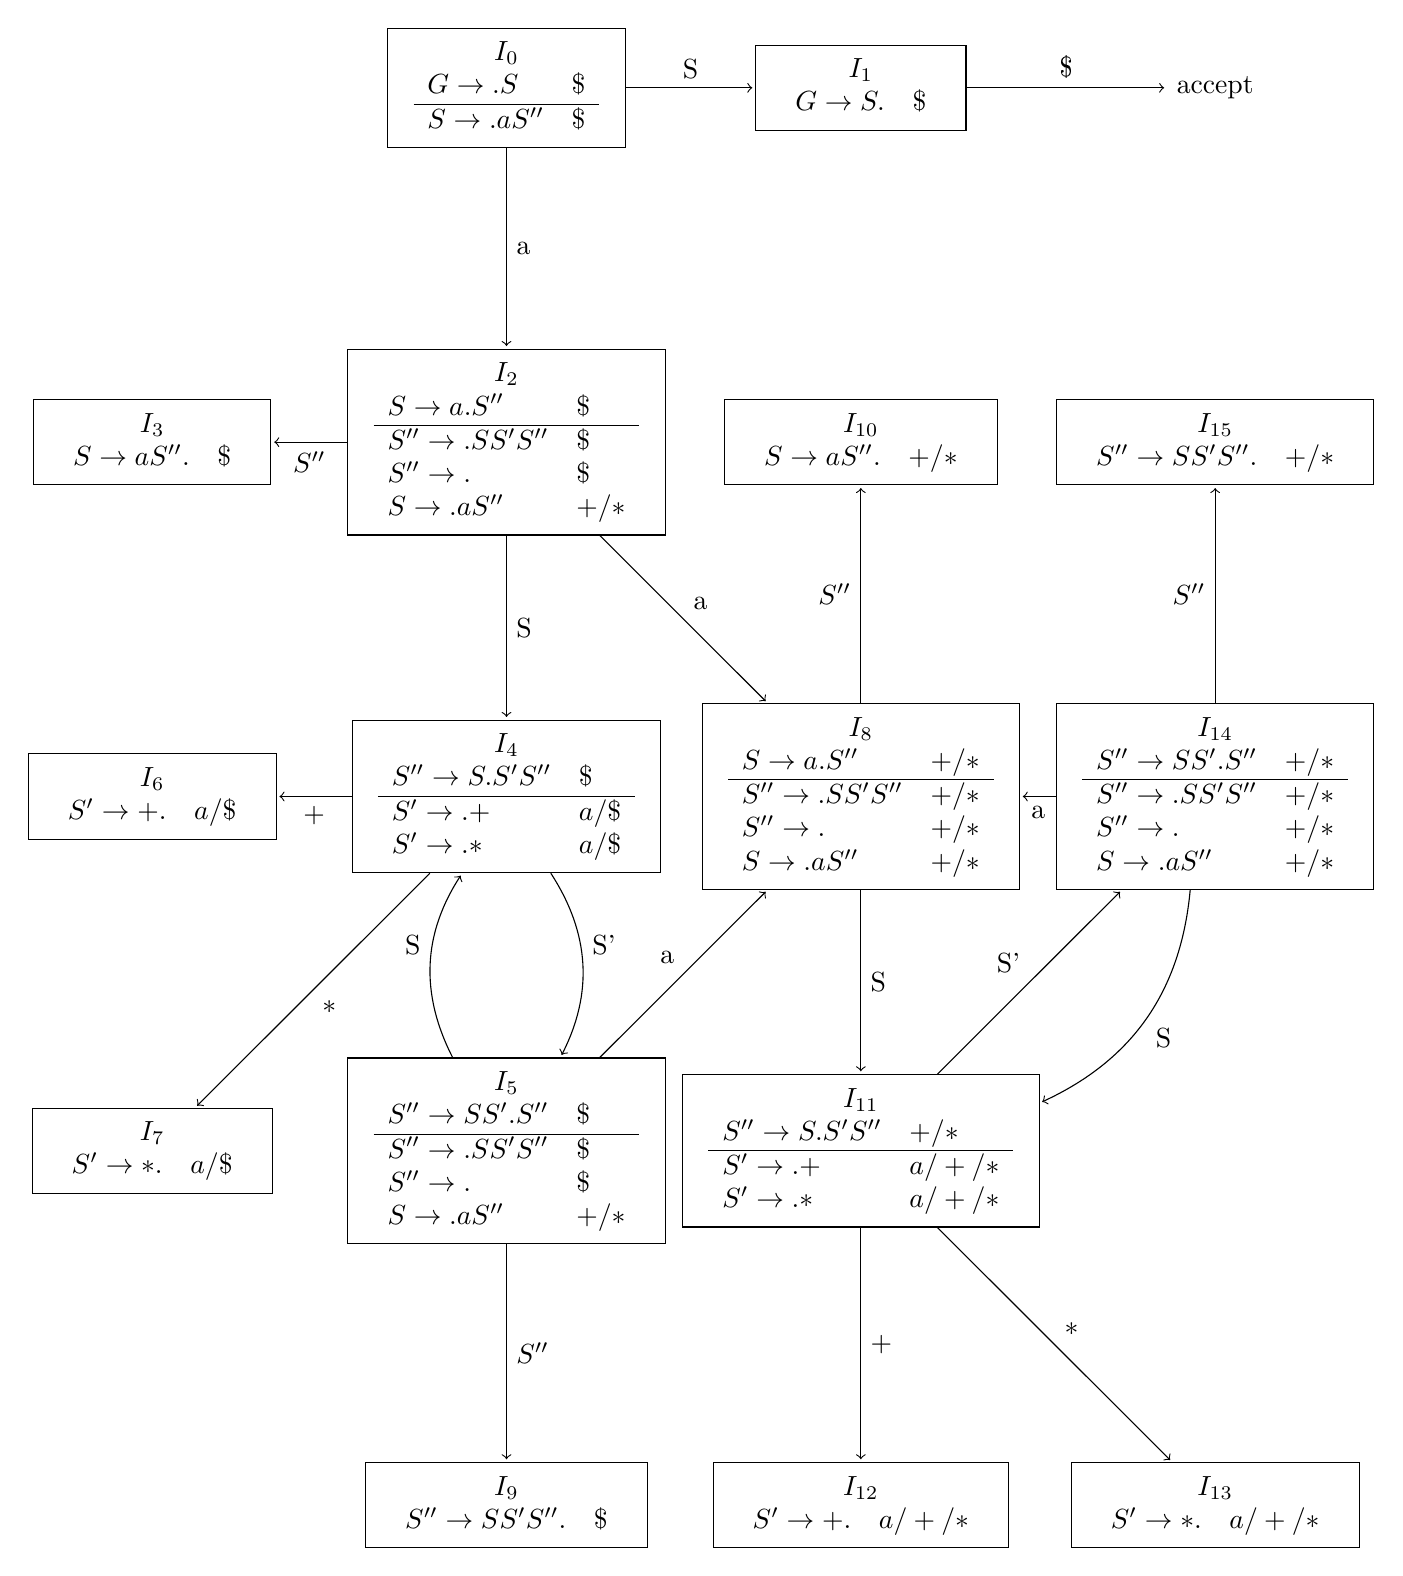
\begin{tikzpicture}[shorten >= 1pt, node distance = 4.5cm, on grid, auto]
  \node[state, rectangle] (0) {
    \begin{tabular}{c} $I_0$ \\
      $\begin{array}{ll} 
        G \rightarrow .S &\$ \\
        \hline
        S \rightarrow .aS^{\prime\prime} &\$ \\
      \end{array}$
    \end{tabular}};
  \node[state, rectangle] [right=of 0] (1) {
    \begin{tabular}{c} $I_1$ \\ 
      $\begin{array}{ll} 
        G \rightarrow S. &\$ \\
      \end{array}$
    \end{tabular}};
  \node[state, rectangle] [below=of 0] (2) {
    \begin{tabular}{c} $I_2$ \\
      $\begin{array}{ll} 
        S \rightarrow a.S^{\prime\prime} &\$ \\
        \hline
        S^{\prime\prime} \rightarrow .SS'S^{\prime\prime} &\$ \\
        S^{\prime\prime} \rightarrow . &\$ \\
        S \rightarrow .aS^{\prime\prime} &+/* \\
      \end{array}$
    \end{tabular}};
  \node[state, rectangle] [left=of 2] (3) {
    \begin{tabular}{c} $I_3$ \\ 
      $\begin{array}{ll} 
        S \rightarrow aS^{\prime\prime}. &\$ \\
      \end{array}$
    \end{tabular}};
  \node[state, rectangle] [below=of 2] (4) {
    \begin{tabular}{c} $I_4$ \\
      $\begin{array}{ll} 
        S^{\prime\prime} \rightarrow S.S'S^{\prime\prime} &\$ \\
        \hline
        S' \rightarrow .+ &a/\$ \\
        S' \rightarrow .* &a/\$ \\
      \end{array}$
    \end{tabular}};
  \node[state, rectangle] [below=of 4] (5) {
    \begin{tabular}{c} $I_5$ \\
      $\begin{array}{ll} 
        S^{\prime\prime} \rightarrow SS'.S^{\prime\prime} &\$ \\
        \hline
        S^{\prime\prime} \rightarrow .SS'S^{\prime\prime} &\$ \\
        S^{\prime\prime} \rightarrow . &\$ \\
        S \rightarrow .aS^{\prime\prime} &+/* \\
      \end{array}$
    \end{tabular}};
  \node[state, rectangle] [left=of 4] (6) {
    \begin{tabular}{c} $I_6$ \\ 
      $\begin{array}{ll} 
        S' \rightarrow +. &a/\$ \\
      \end{array}$
    \end{tabular}};
  \node[state, rectangle] [below=of 6] (7) {
    \begin{tabular}{c} $I_7$ \\ 
      $\begin{array}{ll} 
        S' \rightarrow *. &a/\$ \\
      \end{array}$
    \end{tabular}};
  \node[state, rectangle] [right=of 4] (8) {
    \begin{tabular}{c} $I_8$ \\
      $\begin{array}{ll} 
        S \rightarrow a.S^{\prime\prime} &+/* \\
        \hline
        S^{\prime\prime} \rightarrow .SS'S^{\prime\prime} &+/* \\
        S^{\prime\prime} \rightarrow . &+/* \\
        S \rightarrow .aS^{\prime\prime} &+/* \\
      \end{array}$
    \end{tabular}};
  \node[state, rectangle] [below=of 5] (9) {
    \begin{tabular}{c} $I_9$ \\ 
      $\begin{array}{ll} 
        S^{\prime\prime} \rightarrow SS'S^{\prime\prime}. &\$ \\
      \end{array}$
    \end{tabular}};
  \node[state, rectangle] [above=of 8] (10) {
    \begin{tabular}{c} $I_{10}$ \\ 
      $\begin{array}{ll} 
        S \rightarrow aS^{\prime\prime}. &+/* \\
      \end{array}$
    \end{tabular}};
  \node[state, rectangle] [below=of 8] (11) {
    \begin{tabular}{c} $I_{11}$ \\ 
      $\begin{array}{ll} 
        S^{\prime\prime} \rightarrow S.S'S^{\prime\prime} &+/* \\
        \hline
        S' \rightarrow .+ &a/+/* \\
        S' \rightarrow .* &a/+/* \\
      \end{array}$
    \end{tabular}};
  \node[state, rectangle] [below=of 11] (12) {
    \begin{tabular}{c} $I_{12}$ \\ 
      $\begin{array}{ll} 
        S' \rightarrow +. &a/+/* \\
      \end{array}$
    \end{tabular}};
  \node[state, rectangle] [right=of 12] (13) {
    \begin{tabular}{c} $I_{13}$ \\ 
      $\begin{array}{ll} 
        S' \rightarrow *. &a/+/* \\
      \end{array}$
    \end{tabular}};
  \node[state, rectangle] [right=of 8] (14) {
    \begin{tabular}{c} $I_{14}$ \\
      $\begin{array}{ll} 
        S^{\prime\prime} \rightarrow SS'.S^{\prime\prime} &+/* \\
        \hline
        S^{\prime\prime} \rightarrow .SS'S^{\prime\prime} &+/* \\
        S^{\prime\prime} \rightarrow . &+/* \\
        S \rightarrow .aS^{\prime\prime} &+/* \\
      \end{array}$
    \end{tabular}};
  \node[state, rectangle] [above=of 14] (15) {
    \begin{tabular}{c} $I_{15}$ \\
      $\begin{array}{ll} 
        S^{\prime\prime} \rightarrow SS'S^{\prime\prime}. &+/* \\
      \end{array}$
    \end{tabular}};
  \node[] (100) [right=of 1] {accept};
  \path[->]
    (0) edge node {S} (1)
        edge node {a} (2)
    (2) edge node {$S^{\prime\prime}$} (3)
        edge node {S} (4)
        edge node {a} (8)
    (4) edge node {+} (6)
        edge node {$*$} (7)
        edge [bend left] node {S'} (5)
    (5) edge [bend left] node {S} (4)
        edge node {$S^{\prime\prime}$} (9)
        edge node {a} (8)
    (8) edge node {$S^{\prime\prime}$} (10)
        edge node {S} (11)
    (11) edge node {+} (12)
         edge node {$*$} (13)
         edge node {S'} (14)
    (14) edge node {a} (8)
         edge [bend left] node {S} (11)
         edge node {$S^{\prime\prime}$} (15)
    (1) edge node {\$} (100);
\end{tikzpicture}
\end{document}
